% id: 129-49
% book: 베이직쎈 대수 · 07 삼각함수의 그래프
% section: 개념 47 삼각방정식
% passage: 다음 방정식을 푸시오.
% figure: none
% answer: 
% answer_source: 
% variant_level: 0 (원본 전사)
% 이 파일은 build.mjs 가 items.json 에서 만든다. 고칠 때는 items.json 을 고친다.
\smash{\raisebox{4.5mm}{\dmkichul{베이직쎈 대수 129쪽 49번}}}
$\sin x=\dfrac{1}{2}$ \dmcondfill{$0\le x<2\pi$}{}
\dmhint{주어진 방정식의 해는 함수 $y=\sin x\ (0\le x<2\pi)$의 그래프와 직선 $y=\blank$의 교점의 $x$좌표와 같다.\par\smallskip\dispeq{% 129-49(129쪽) — 🎯 힌트 안 그래프: $y=\sin x$ $(0\le x<2\pi)$ 의 그래프와 직선 $y=\frac{1}{2}$.
% 스캔 화질이 낮아 TikZ 로 다시 그림. 라벨은 원문에 있는 것만 — $y$축 $1$·$-1$, $x$축 $\frac{\pi}{2}$·$\pi$·$\frac{3}{2}\pi$·$2\pi$.
% 교점의 $x$좌표(= 이 문항의 답)는 원문에도 적혀 있지 않으므로 점만 찍고 값은 쓰지 않는다.
\begin{tikzpicture}[line width=0.6pt, x=0.80cm, y=0.72cm]
  \draw[dotted, line width=0.5pt] (0,1) -- (1.5708,1) (1.5708,0) -- (1.5708,1);
  \draw[dotted, line width=0.5pt] (0,-1) -- (4.7124,-1) (4.7124,0) -- (4.7124,-1);
  \draw[dotted, line width=0.5pt] (6.2832,0) -- (6.2832,0.5);
  \draw[->, >=stealth, line width=0.7pt] (-0.65,0) -- (7.45,0) node[below=1pt, font=\footnotesize] {$x$};
  \draw[->, >=stealth, line width=0.7pt] (0,-1.70) -- (0,1.80) node[left=1pt, font=\footnotesize] {$y$};
  \draw[line width=0.6pt] (-0.65,0.5) -- (7.05,0.5);
  \draw[line width=0.7pt, domain=0:6.2832, samples=140, smooth] plot (\x, {sin(57.2958*\x)});
  \fill (0,0) circle (1.7pt);
  \draw[fill=white, line width=0.5pt] (6.2832,0) circle (1.7pt);
  \fill[red!75] (0.5236,0.5) circle (1.7pt);
  \fill[red!75] (2.6180,0.5) circle (1.7pt);
  \node[anchor=east, font=\footnotesize] at (-0.12,1) {$1$};
  \node[anchor=east, font=\footnotesize] at (-0.12,-1) {$-1$};
  \node[anchor=north east, font=\footnotesize] at (-0.04,-0.06) {$\pt{O}$};
  \node[anchor=north, font=\footnotesize] at (1.5708,-0.10) {$\dfrac{\pi}{2}$};
  \node[anchor=south, font=\footnotesize, fill=white, inner sep=0.6pt] at (3.1416,0.05) {$\pi$};
  \node[anchor=north west, font=\footnotesize] at (5.00,-0.52) {$\dfrac{3}{2}\pi$};
  \draw[->, >=stealth, line width=0.4pt] (5.00,-0.56) -- (4.77,-0.10);
  \node[anchor=south east, font=\footnotesize, fill=white, inner sep=0.6pt] at (6.55,0.05) {$2\pi$};
  \node[anchor=south west, font=\footnotesize] at (0.95,1.04) {$y=\sin x$};
  \node[anchor=south east, font=\footnotesize] at (7.00,0.56) {$y=\dfrac{1}{2}$};
\end{tikzpicture}
}\par\smallskip\noindent 따라서 구하는 해는 \quad $x=\blank$ 또는 $x=\blank[2.4em]$}
